% !TEX program = xelatex
% AY2022 材料力学 解答例（同志社 生命医科学 医工学コース 院試）
% 問題・図は 01_exams/2022/tex を土台に、参考/ の粒度で解答を付した。
\documentclass[11pt,a4paper]{article}
\usepackage{../../00_common/preamble}
\usetikzlibrary{positioning,arrows.meta,calc,patterns,decorations.pathmorphing}
\newcommand{\maru}[1]{\tikz[baseline=(c.base)]{\node[circle,draw,inner sep=0.4pt,minimum size=1.1em](c){\scriptsize #1};}}

\title{材料力学 AY2022 解答例}
\author{}
\date{}

\begin{document}
\maketitle

\noindent\textbf{符号規約}：〔I〕では上向きの変位および引張応力を正とする
（圧縮は負）．〔II〕では座標 $z$ の上向きを正とし，集中荷重 $P$ は下向き（$-z$）とする．
曲げ応力は引張側を正，たわみ・変位は荷重の向き（下向き）を正の大きさとして表す．

%====================================================================
\section*{〔I〕}

図1のように，下側を床に固定した 2 本の棒\maru{1}および 1 本の棒\maru{2}があり，
上側を剛体板に接合する．棒\maru{2}の中央（点 a）に外力 $P$ が下向きに作用し，
棒\maru{2}の温度のみ $\Delta T$ 上昇させる（床・剛体板は断熱で棒\maru{1}の温度は不変）．
初期長さ $L$，断面積 $A$，縦弾性係数はそれぞれ $E$（棒\maru{1}），$2E$（棒\maru{2}），
線膨張係数はともに $\alpha$，剛体板は床と平行を保って変位する．

\begin{center}
\begin{tikzpicture}[>=Latex,scale=1.0]
  \fill[pattern=north east lines] (-0.2,-1.0) rectangle (6.2,0); \draw (-0.2,0) -- (6.2,0);
  \fill[gray!70] (0.2,4.0) rectangle (6.4,4.5);
  \node[right] at (6.45,4.25) {剛体板};
  \draw (0.7,0) rectangle (1.2,4.0);
  \fill[gray!30] (2.7,0) rectangle (3.3,4.0); \draw (2.7,0) rectangle (3.3,4.0);
  \draw (5.0,0) rectangle (5.5,4.0);
  \node[above] at (0.95,4.0) {棒\maru{1}}; \node[above] at (3.0,4.0) {棒\maru{2}}; \node[above] at (5.25,4.0) {棒\maru{1}};
  \draw[->,very thick] (3.0,2.0) -- (3.0,0.6) node[pos=0.35,left,fill=white,inner sep=1pt]{$P$};
  \node[right] at (3.35,2.0) {a};
  \draw[->] (6.0,0) -- (6.0,1.5) node[left]{$x$};
  \node[right] at (6.45,-0.5) {床};
  \draw[<->] (0.35,0) -- (0.35,4.0) node[midway,fill=white]{$L$};
  \draw[<->] (2.2,0) -- (2.2,2.0) node[midway,fill=white,inner sep=1pt,font=\scriptsize]{$L/2$};
\end{tikzpicture}

\vspace{1mm}
図1
\end{center}

\begin{enumerate}[label=(\arabic*)]
  \item 棒\maru{1}と棒\maru{2}に生じる応力 $\sigma_1$ と $\sigma_2$ を求めよ.
  \item 棒\maru{2}における点 a の変位 $\lambda_a$ を求めよ.
  \item 剛体板の変位 $\lambda$ が $\lambda=0$ となる $P$ を求めよ.
\end{enumerate}

\subsection*{解答}

\noindent\textbf{モデル化}\quad 剛体板は床と平行を保って変位するので，
3 本の棒の上端変位はすべて等しい．これを $\lambda$（上向き正）とおく．
棒\maru{2}は点 a に荷重 $P$ を受けるため，下半区間（床$\to$a）と上半区間（a$\to$板）で
内力が異なる．点 a の変位を $\lambda_a$（上向き正）とおく．内力は引張を正とする．

各棒の剛性は
\[
  \frac{EA}{L}\ (\text{棒\maru{1}}),\qquad
  \frac{(2E)A}{L/2}=\frac{4EA}{L}\ (\text{棒\maru{2}の各半区間}).
\]
棒\maru{2}の各半区間の自由熱伸びは $\alpha\,\Delta T\,(L/2)$ である．
よって各内力は，伸び＝（弾性伸び）＋（熱伸び）の関係から

\noindent{}棒\maru{1}（熱変化なし，伸び $\lambda$）：
\[
  N_1=\frac{EA}{L}\,\lambda .
\]
棒\maru{2}上半（伸び $\lambda-\lambda_a$）・下半（伸び $\lambda_a$）：
\[
  N_{2u}=\frac{4EA}{L}\!\left(\lambda-\lambda_a-\tfrac{\alpha\,\Delta T\,L}{2}\right),\qquad
  N_{2\ell}=\frac{4EA}{L}\!\left(\lambda_a-\tfrac{\alpha\,\Delta T\,L}{2}\right).
\]

\medskip
\noindent\textbf{つり合い式}\quad 剛体板（外力なし，棒\maru{1}が 2 本と棒\maru{2}上半が接合）と，
節点 a（外力 $P$ 下向き）について，鉛直方向のつり合いより
\[
  2N_1+N_{2u}=0, \qquad N_{2u}-N_{2\ell}-P=0 .
\]

\medskip
\noindent\textbf{(1)}\quad 上の 2 式に内力を代入すると
\[
  3\lambda-2\lambda_a-\alpha\,\Delta T\,L=0,\qquad
  \frac{4EA}{L}\,(\lambda-2\lambda_a)=P .
\]
これを解いて
\[
  \lambda=\frac{\alpha\,\Delta T\,L}{2}-\frac{PL}{8EA},\qquad
  \lambda_a=\frac{\alpha\,\Delta T\,L}{4}-\frac{3PL}{16EA}.
\]
よって応力 $\sigma_1=N_1/A$, $\sigma_2=N_2/A$ は
\[
  \ans{\;\sigma_1=\frac{E\,\alpha\,\Delta T}{2}-\frac{P}{8A}\;}
\]
\[
  \ans{\;\sigma_{2}^{\text{(上半)}}=-E\,\alpha\,\Delta T+\frac{P}{4A},\qquad
        \sigma_{2}^{\text{(下半)}}=-E\,\alpha\,\Delta T-\frac{3P}{4A}\;}
\]
（棒\maru{2}は点 a を境に内力が変わるため，上半・下半で応力が異なる．負は圧縮を表す．）

検算：床に伝わる軸力の和は $2N_1+N_{2\ell}=-P$，すなわち床は合計 $P$ を上向きに支える．
これは外力 $P$（下向き）とつり合う $\checkmark$．

\medskip
\noindent\textbf{(2)}\quad (1) で求めた点 a の変位は
\[
  \ans{\;\lambda_a=\frac{\alpha\,\Delta T\,L}{4}-\frac{3PL}{16EA}\;}
\]
（上向き正．第 1 項は熱膨張による上昇，第 2 項は荷重 $P$ による下降を表す．）

\medskip
\noindent\textbf{(3)}\quad 剛体板の変位は $\displaystyle\lambda=\frac{\alpha\,\Delta T\,L}{2}-\frac{PL}{8EA}$．
$\lambda=0$ より
\[
  \frac{\alpha\,\Delta T\,L}{2}=\frac{PL}{8EA}
  \;\Longrightarrow\;
  \ans{\;P=4EA\,\alpha\,\Delta T\;}
\]
検算：この $P$ を $\lambda$ に代入すると
$\dfrac{\alpha\Delta T L}{2}-\dfrac{(4EA\alpha\Delta T)L}{8EA}
=\dfrac{\alpha\Delta T L}{2}-\dfrac{\alpha\Delta T L}{2}=0$ $\checkmark$．

%====================================================================
\clearpage
\section*{〔II〕}

図2のように，長さ $L$ の丸棒（直径 $d$）は点 A で固定され，他端 B に長さ $L/3$ の剛体棒が
接合されている．丸棒の先端 B に下向きに集中荷重 $P$ が作用し，同時に剛体棒の先端 C にも
下向きに集中荷重 $P$ が作用する．丸棒の縦弾性係数を $E$，横弾性係数を $G$ とする．

\begin{center}
\begin{tikzpicture}[>=Latex]
  \fill[pattern=north east lines] (0.2,0.6) -- (0.2,3.0) -- (1.2,3.4) -- (1.2,1.0) -- cycle;
  \draw (0.2,0.6) -- (0.2,3.0) -- (1.2,3.4) -- (1.2,1.0) -- cycle;
  \draw[line width=12pt,gray!25,line cap=round] (0.9,2.4) -- (6.0,1.0);
  \draw[fill=gray!25] (6.0,1.0) ellipse (0.32 and 0.12);
  \draw[line width=2pt] (6.0,0.95) -- (8.3,1.5);
  \draw[->] (0.9,2.4) -- (0.9,3.7) node[left]{$z$};
  \draw[->] (0.9,2.4) -- (2.0,2.95) node[above]{$y$};
  \draw[->] (0.9,2.4) -- (2.0,1.95) node[below]{$x$};
  \node[left] at (0.8,2.35) {A}; \node[below] at (6.0,0.75) {B}; \node[right] at (8.35,1.5) {C};
  \fill (2.3,2.25) circle (1.8pt); \node[above] at (2.3,2.3) {u};
  \draw[->,very thick] (6.0,2.1) -- (6.0,1.15); \node[right] at (6.05,1.95) {$P$};
  \draw[->,very thick] (8.3,2.55) -- (8.3,1.6); \node[right] at (8.35,2.4) {$P$};
  \draw[<->] (1.1,3.05) -- (6.0,1.65) node[midway,above,font=\scriptsize]{$L$};
  \draw[<->] (1.0,1.95) -- (2.3,1.6) node[midway,below,font=\scriptsize]{$L/4$};
  \draw[<->] (6.1,0.65) -- (8.3,1.2) node[midway,below,font=\scriptsize]{$L/3$};
  \begin{scope}[shift={(0.9,-1.5)}]
    \draw (0,0) circle (0.55);
    \draw[->] (0,-0.85) -- (0,0.95) node[right]{$z$};
    \draw[->] (-0.85,0) -- (0.95,0) node[above]{$y$};
    \fill (0,0.55) circle (1.8pt); \node[above left] at (0,0.55) {u};
    \node at (0,-1.25) {\underline{断面}};
  \end{scope}
\end{tikzpicture}

\vspace{1mm}
図2
\end{center}

\begin{enumerate}[label=(\arabic*)]
  \item 固定端 A での支持力 $R_a$, 支持モーメント $M_a$, 支持トルク $T_a$ を図示し, 数式で示せ.
  \item 丸棒のせん断力図（SFD）と曲げモーメント図（BMD）を求めて, 図示せよ.
  \item 固定端 A から $L/4$ の位置にある断面の点 u の $\sigma_x$, $\sigma_y$, $\tau_{xy}$ を求めよ.
  \item 点 B および C の $z$ 方向の変位 $\delta_B$, $\delta_C$ を求めよ. ただし,
        断面二次モーメントを $I$, 断面二次極モーメントを $I_p$ とする.
\end{enumerate}

\subsection*{解答}

\noindent\textbf{座標設定}\quad A を原点に，丸棒の軸方向を $x$（A$\to$B），$y$ を剛体棒の方向，
$z$ を上向きにとる．B の位置は $(L,0,0)$，C の位置は $(L,\,L/3,\,0)$．
荷重は B と C にそれぞれ $(0,0,-P)$．

\medskip
\noindent\textbf{(1)}\quad 鉛直方向の力のつり合いより支持力は荷重の総和に等しく
$R_a=2P$（上向き）．固定端 A まわりのモーメントのつり合いを各荷重の
位置ベクトルとの外積でとると
\[
  \sum \boldsymbol r\times\boldsymbol F
  =(L,0,0)\times(0,0,-P)+(L,\tfrac{L}{3},0)\times(0,0,-P)
  =\Big(-\tfrac{PL}{3},\,2PL,\,0\Big).
\]
これと反力モーメント $\boldsymbol M_a$ がつり合うので
$\boldsymbol M_a=\big(\tfrac{PL}{3},\,-2PL,\,0\big)$．
$x$ 成分は棒軸まわり（トルク），$y$ 成分は曲げモーメントである．
C 点荷重が軸から $L/3$ 偏心することがトルクの源である．
\[
  \ans{\;R_a=2P\ (\text{上向き}),\quad
        M_a=2PL\ (y\text{軸まわりの曲げ}),\quad
        T_a=\frac{PL}{3}\ (x\text{軸まわりのトルク})\;}
\]

\medskip
\noindent\textbf{(2)}\quad 丸棒の任意断面 $x$（A から測る）の右側には B 点荷重 $P$ と C 点荷重 $P$ があり，
両者とも軸座標は $x=L$．よってせん断力は一定，曲げモーメントは断面から $B$ までの距離に比例する．
\[
  \ans{\;Q(x)=2P\ (\text{一定}),\qquad M(x)=2P\,(L-x)\;}
\]
端点の値：$M(0)=2PL$，$M(L)=0$．また C 点荷重の偏心により軸全長に一定トルク $T=PL/3$ が働く．

\begin{center}
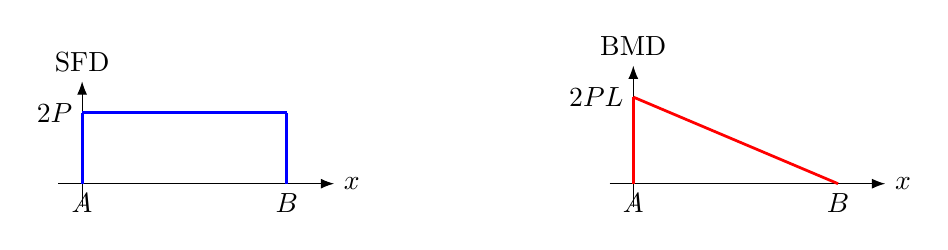
\begin{tikzpicture}[>=Latex,scale=1.0]
  \def\L{2.6}
  \begin{scope}
    \draw[->] (-0.3,0) -- (\L+0.6,0) node[right]{$x$};
    \draw[->] (0,-0.3) -- (0,1.3) node[above]{SFD};
    \draw[line width=1pt,blue] (0,0.9) -- (\L,0.9);
    \draw[line width=1pt,blue] (0,0)--(0,0.9); \draw[line width=1pt,blue] (\L,0.9)--(\L,0);
    \node[left] at (0,0.9) {$2P$};
    \node[below] at (0,0) {$A$}; \node[below] at (\L,0) {$B$};
  \end{scope}
  \begin{scope}[xshift=7.0cm]
    \draw[->] (-0.3,0) -- (\L+0.6,0) node[right]{$x$};
    \draw[->] (0,-0.3) -- (0,1.5) node[above]{BMD};
    \draw[line width=1pt,red] (0,1.1) -- (\L,0);
    \draw[line width=1pt,red] (0,0)--(0,1.1);
    \node[left] at (0,1.1) {$2PL$};
    \node[below] at (0,0) {$A$}; \node[below] at (\L,0) {$B$};
  \end{scope}
\end{tikzpicture}
\end{center}

\medskip
\noindent\textbf{(3)}\quad $x=L/4$ の断面の曲げモーメントは
$M=2P\!\left(L-\tfrac{L}{4}\right)=\tfrac{3PL}{2}$．
点 u は断面の上面（$z=+d/2$，中立軸 $y$ 軸から最遠の繊維）にある．
片持ち梁で下向き荷重を受けるため上面は引張．曲げ応力は
\[
  \sigma_x=\frac{M\,(d/2)}{I}=\frac{(3PL/2)(d/2)}{I}=\frac{3PLd}{4I}.
\]
$y$ 方向には荷重がなく単軸曲げなので $\sigma_y=0$．
せん断応力はトルク $T=PL/3$ による表面せん断が寄与する
（横せん断力 $Q$ 由来の応力は最遠繊維 u では 0）．
点 u（上面）でねじりせん断は周方向（$\pm y$）を向くので $\tau_{xy}$ となり
\[
  \tau_{xy}=\frac{T\,(d/2)}{I_p}=\frac{(PL/3)(d/2)}{I_p}=\frac{PLd}{6I_p}.
\]
\[
  \ans{\;\sigma_x=\frac{3PLd}{4I},\qquad \sigma_y=0,\qquad \tau_{xy}=\frac{PLd}{6I_p}\;}
\]
検算：$M(L/4)=2P(L-L/4)=\tfrac{3}{2}PL$，$M(0)=2PL$ から線形補間しても一致 $\checkmark$．

\medskip
\noindent\textbf{(4)}\quad 丸棒は A で固定された片持ち梁とみなせる．先端 B には
B 点荷重 $P$ と剛体棒を介した C 点荷重 $P$ が伝わり，合計の横荷重 $2P$ が先端に作用する
（C 荷重は B と同じ軸座標なので $y$ 軸まわりの付加曲げモーメントは生じない）．
よって B の曲げたわみは
\[
  \delta_B=\frac{(2P)L^3}{3EI}=\frac{2PL^3}{3EI}.
\]
C は剛体棒で B につながる．C の $z$ 変位は，B の並進 $\delta_B$ に，
トルクによる丸棒のねじれ角 $\theta$ ぶんの剛体棒（長さ $L/3$）の回転が加わる．
\[
  \theta=\frac{T\,L}{G\,I_p}=\frac{(PL/3)L}{GI_p}=\frac{PL^2}{3GI_p},\qquad
  \delta_C=\delta_B+\theta\cdot\frac{L}{3}.
\]
\[
  \ans{\;\delta_B=\frac{2PL^3}{3EI}\ (\text{下向き})\;}
\]
\[
  \ans{\;\delta_C=\frac{2PL^3}{3EI}+\frac{PL^3}{9GI_p}\ (\text{下向き})\;}
\]
検算：$\delta_C-\delta_B=\theta\cdot\dfrac{L}{3}=\dfrac{PL^2}{3GI_p}\cdot\dfrac{L}{3}
=\dfrac{PL^3}{9GI_p}>0$．ねじれによる回転で C 側が B より余分に下がることと整合する $\checkmark$．

\end{document}
